\documentclass{article}

%%% SOME USEFUL PACKAGES %%%
\usepackage[english]{babel} % hyphenation
\usepackage[margin=1.5cm]{geometry} % margins
\usepackage{graphicx} % support for graphics
\usepackage{amsmath} % support for math­e­mat­i­cal typesetting
\usepackage{amssymb} % math­e­mat­i­cal symbols
\usepackage{color} % support for colors
\usepackage{mathtools} % more math­e­mat­i­cal type­set­ting
\usepackage{amsthm} % for defining theorem-like environments
\usepackage{enumerate} % change appearance of numbered lists
\usepackage{framed} % textboxes
\usepackage[format=plain,labelfont=bf,up]{caption} % cus­tomise cap­tions for fig­ures and ta­bles
\usepackage[colorlinks=true,linkcolor=black,urlcolor=blue,linktoc=all, citecolor=black]{hyperref} % hyperlinks
\usepackage{setspace}
\usepackage{verbatim}

%%% CUSTOM COMMANDS %%%
\def\ci{\perp\!\!\!\perp} % statistical independence symbol
\newcommand{\ind}{1\hspace{-2.1mm}{1}} % indicator function
\newcommand{\rl}{\mathbb{R}} % real numbers
\newcommand{\ex}[1]{\mathbb{E} \left\{ #1 \right\}} % expectation operator
\newcommand{\pr}[1]{\mathbb{P} \left\{ #1 \right\}} % probability
\newcommand{\var}[1]{\mathbb{V}\text{ar} \left\{ #1 \right\}} % variance
\newcommand{\cov}[1]{\mathbb{C}{ov} \left\{ #1 \right\}} % covariance
\newcommand{\corr}[1]{\mathbb{C}{orr} \left\{ #1 \right\}} % correlation
\newcommand{\inprod}[1]{\langle #1 \rangle}

\begin{document}
	\title{OSM Lab 2017: Math Pset 6}
	\author{Wei Han Chia}
	\date{Due: 31 July 2017}
	\maketitle
	
	\section*{Problems from the Book}
	\subsection*{8.1}
	We can plot the feasible set. Further, we note that the objective function is decreasing in y and increasing in x, and so our optimizer for this problem is (2.8, 3.2).
	
	\begin{figure}[!h]
		\centering
		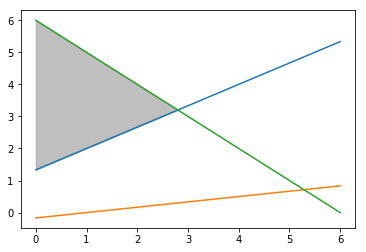
\includegraphics[scale = 0.5]{fig1}
		\caption{Feasible Set of 8.1}
	\end{figure}
	
	\subsection*{8.2}
	(i) We can draw the feasible polygon. Checking the value of the function at each of the vertices yields a maximum at (6,2), with function value 20.
	
	\begin{figure}[!h]
		\centering
		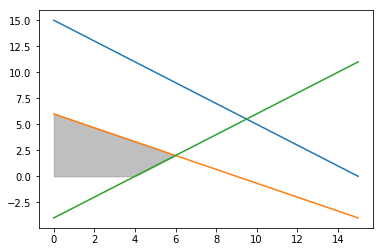
\includegraphics[scale = 0.5]{fig2}
		\caption{FeasibleSet of 8.2(i)}
	\end{figure}
	\newpage
	(ii) We can draw the feasible polygon. Checking the value of the function at each of the vertices yields a maximum at (15, 12), with function value 132.
	
	\begin{figure}[!h]
		\centering
		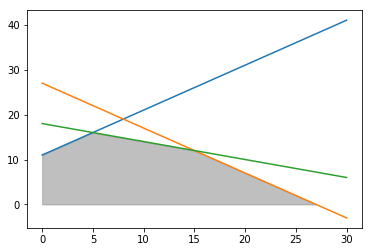
\includegraphics[scale = 0.5]{fig3}
		\caption{FeasibleSet of 8.2(ii)}
	\end{figure}
	
	\subsection*{8.5}
	
	(i)
	
	\begin{figure}[!h]
		\begin{tabular}{c c c c c c c}
			$z$ & = & & & $3x_1$ & + & $x_2$ \\
			\hline
			$w_1$ & = & 15 & - &$x_1$& - &$3x_2$ \\
			$w_2$ & = & 18 & - & $2x_1$ & - & $3x_2$ \\
			$w_3$ & = & 4 & - & $x_1$ & + & $x_2 $ \\
			\hline
		\end{tabular}
	\end{figure}
	
	\begin{figure}[!h]
		\begin{tabular}{c c c c c c c}
			$z$ & = &12 &- & $3w_3$ & + & $4x_2$ \\
			\hline
			$w_1$ & = & 11 & + &$w_3$& - &$4x_2$ \\
			$w_2$ & = & 10 & + & $2w_3$ & - & $5x_2$ \\
			$x_1$ & = & 4 & - & $w_3$ & + & $x_2 $ \\
			\hline
		\end{tabular}
	\end{figure}
	
	\begin{figure}[!h]
		\begin{tabular}{c c c c c c c}
			$z$ & = & 20 &- & $7/5 w_3$ &  - & $4/5 w_2$ \\
			\hline
			$w_1$ & = & 3 & - &$3/5 w_3$& + &$1/5 w_2$ \\
			$x_2$ & = & 2 & + & $2/5 w_3$ & - & $1/5 w_2$ \\
			$x_1$ & = & 6 & - & $3/5 w_3$ & - & $1/5 w_2 $ \\
			\hline
		\end{tabular}
	\end{figure}
	So our solution is indeed (6,2) with function value 20.
	
	(ii)
	\begin{figure}[!h]
		\begin{tabular}{c c c c c c c}
			$z$ & = & & & $4x_1$ & + & $6x_2$ \\
			\hline
			$w_1$ & = & 11 & + &$x_1$& - &$x_2$ \\
			$w_2$ & = & 27 & - & $x_1$ & - & $x_2$ \\
			$w_3$ & = & 90 & - & $2x_1$ & - & $5x_2 $ \\
			\hline
		\end{tabular}
	\end{figure}
	
	\begin{figure}[!h]
		\begin{tabular}{c c c c c c c}
			$z$ & = & 66 & + & $10x_1$ & - & $6w_1$ \\
			\hline
			$x_2$ & = & 11 & + &$x_1$& - &$w_1$ \\
			$w_2$ & = & 16 & - & $2 x_1$ & + & $w_1$ \\
			$w_3$ & = & 35 & - & $7 x_1$ & + & $5w_1 $ \\
			\hline
		\end{tabular}
	\end{figure}	

	\begin{figure}[!h]
		\begin{tabular}{c c c c c c c}
			$z$ & = & 116 & - & $10/7 w_3 $ & - & $8/7 w_1$ \\
			\hline
			$x_2$ & = & 16 & - &$1/7 w_3 $& - &$2/7 w_1$ \\
			$w_2$ & = & 6 & + & $2/7 w_3 $ & + & $3/7 w_1$ \\
			$x_1$ & = & 5 & - & $1/7 w_3$ & + & $5/7 w_1 $ \\
			\hline
		\end{tabular}
	\end{figure}	

	\newpage
	\begin{figure}[!h]
		\begin{tabular}{c c c c c c c}
			$z$ & = & 132 & - & $2/3 w_3 $ & - & $8/3 w_2$ \\
			\hline
			$x_2$ & = & 12 & - &$1/3 w_3 $& - &$2/3 w_2$ \\
			$w_2$ & = & 14 & + & $2/3 w_3 $ & + & $7/3 w_2$ \\
			$x_1$ & = & 15 & + & $1/3 w_3$ & - & $5/3 w_2 $ \\
			\hline
		\end{tabular}
	\end{figure}	
	
	So our solution is indeed (15, 12) with function value 132.
		
	\subsection*{8.7}
	(i) We note that starting at the origin here is unfeasible. So we first solve the auxiliary problem to get the initial dictionary.

	\begin{figure}[!h]
		\begin{tabular}{c c c c c c c}
			$z$ & = & 2 & + & $1.5 x_2 $ & + & $0.25 w_1$ \\
			\hline
			$x_1$ & = & 2 & - &$0.5x_2 $& + &$0.25 w_1$ \\
			$w_2$ & = & 10 & - & $4 x_2 $ & + & $0.5 w_1$ \\
			$w_3$ & = & 1 & + & $0.5 x_2$ & - & $0.25 w_1 $ \\
			\hline
		\end{tabular}
	\end{figure}
	
	\begin{figure}[!h]
		\begin{tabular}{c c c c c c c}
			$z$ & = & 5.75 & - & $0.375w_2 $ & + & $0.4375 w_1$ \\
			\hline
			$x_1$ & = & 0.75 & + &$0.125 w_2$& + &$0.1875w_1$ \\
			$x_2$ & = & 2.5 & - & $0.25 w_2 $ & + & $0.125 w_1$ \\
			$w_3$ & = & 2.25 & - & $0.125 w_2$ & - & $0.1875 w_1 $ \\
			\hline
		\end{tabular}
	\end{figure}	
	 
	 \begin{figure}[!h]
	 	\begin{tabular}{c c c c c c c}
	 		$z$ & = & 11 & - & $2/3 w_2 $ & - & $7/3 w_3$ \\
	 		\hline
	 		$x_1$ & = & 3 &  && - &$w_3$ \\
	 		$x_2$ & = & 4 & - & $1/3 w_2 $ & + & $2/3 w_3$ \\
	 		$w_1$ & = & 12 & - & $2/3 w_2$ & - & $16/3 w_3 $ \\
	 		\hline
	 	\end{tabular}
	 \end{figure}	
	 So our optimal solution is (3,4), with optimal value 11. 
	 
	 (ii) Once again we note that starting at the origin is unfeasible. However, solving the auxiliary problem shows us that this problem is unfeasible, as the optimal solution of the auxiliary problem does have an optimal value of 0.
	 
	 (iii) 
	 
	 \begin{figure}[!h]
	 	\begin{tabular}{c c c c c c c}
	 		$z$ & = & 0 & - & $3x_1 $ & + & $x_2$ \\
	 		\hline
	 		$w_1$ & = & 4 & && - &$x_2$ \\
	 		$w_2$ & = & 6 & + & $2x_1 $ & - & $3x_2$ \\
	 		\hline
	 	\end{tabular}
	 \end{figure}	
	 
	 \begin{figure}[!h]
	 	\begin{tabular}{c c c c c c c}
	 		$z$ & = & 2 & - & $7/3 x_1 $ & - & $1/3 w_2$ \\
	 		\hline
	 		$w_1$ & = & 2 &- & $2/3 x_1$ & + &$1/3 w_2$ \\
	 		$x_2$ & = & 2 & + & $2/3 x_1$ & + & $1/3 w_2$ \\
	 		\hline
	 	\end{tabular}
	 \end{figure}	 
	 
	 So our optimal solution is (0, 2), with optimal value 2.
	 
	 \subsection*{8.13}
	 Consider the linear problem
	 \begin{align*}
	 \text{maximize} \quad &\mathbf{c}^T \mathbf{x} \\
	 \text{s.t} \quad &A \mathbf{x} \preceq \mathbf{0} \\
	 & \mathbf{x} \succeq \mathbf{0}
	 \end{align*}
	 
	 We can also consider the dual to the problem. 
	 
	 \begin{align*}
	 \text{minimize} \quad &0 \\
	 \text{s.t} \quad &A^T \mathbf{y} \succeq c\\
	 &\mathbf{y} \succeq \mathbf{0}
	 \end{align*}
	 
	 Now we know that if $\mathbf{x} = \mathbf{0}$ is the optimal solution to the problem, then it follows that we have a feasible solution to our dual problem. Now if $\mathbf{x} = \mathbf{0}$ is not an optimum point, then our optimum point must be at some $\mathbf{x} > \mathbf{0}$. This would imply that our function value is greater than 0, which means that our dual is unfeasible. From Proposition 8.6.4, we can conclude that this means our primal problem is unbounded. 
	 
	 \subsection*{8.17}
	 Lets consider some linear problem in standard form:
	 \begin{align*}
	 \text{maximize} \quad &\mathbf{c}^T \mathbf{x} \\
	 \text{s.t} \quad &A \mathbf{x} \preceq \mathbf{b} \\
	 & \mathbf{x} \succeq 0
	 \end{align*}
	 From the text, we know that we can write the dual problem as a maximization problem as follows:
	 \begin{align*}
	 \text{maximize} \quad -&\mathbf{b}^T \mathbf{y} \\
	 \text{s.t} \quad &A^T \mathbf{y} \succeq \mathbf{c} \\
	 & \mathbf{y} \succeq 0
	 \end{align*}
	 Now we can use the same reasoning to define the dual to the dual as:
	 \begin{align*}
	 \text{maximize} \quad  &- (-\mathbf{b}^T \mathbf{z}) \\
	 \text{s.t} \quad &(A^T)^T \mathbf{z} \preceq \mathbf{b} \\
	 & \mathbf{z} \succeq 0
	 \end{align*}
	 
	 It is easy to see that solving for $\mathbf{z}$ and $\mathbf{x}$ are essentially the same, i.e. that the dual of the dual of a linear problem is the primal problem.
	 
	 \subsection*{8.18}
	 The dual of the linear problem is as follows:
	 \begin{align*}
	 \text{minimize} \quad & 3y_1 + 5y_2 + 4y_3)\\
	 \text{s.t} \quad & 2y_1 + y_2 + 2y_3 \geq 1 \\
	 & y_1 + 3y_2 + 3y_3 \geq 1 \\
	 &y_1, y_2, y_3 \geq 0
	 \end{align*}
	 
	 Solving the primal problem yields $x_1 = 5/4, x_2 = 1/2$, and a function value of $7/4$. 
	 
	 Solving the dual problem yields $y_1 = 1/4, y_2 = 0, y_3 = 1/4$ and a function value of $7/4$. 
	 
	 So our function values to the primal and dual problems are indeed equal.
	\end{document}